\documentclass[14pt]{beamer}
\usetheme{Warsaw}
\usecolortheme{beaver}
\usefonttheme{professionalfonts}

\input{../../preamble}
\usepackage{amscd,amsmath,amssymb,amsthm,graphicx}
\usepackage[mathscr]{eucal}
\usepackage{paralist}
\usepackage{tabto}
\usepackage[normalem]{ulem}

% % % % % % % % % %
\title[Cal I S2015]{MATH 2554 (Calculus I)}
\subtitle{}
\author[Wheeler]{Dr. Ashley K. Wheeler}
\institute{University of Arkansas}
\date{\today}
\logo{}

% % %
\begin{document}
\maketitle

% % %
\begin{frame}
\frametitle{Table of Contents}
\tableofcontents
\end{frame}

% % % % % % % % % % Wed 21 Jan 2015
\begin{frame}
\section[Week 2]{Week 2: 20-23 January}
\frametitle{Wednesday 21 January (Week 2)}
\begin{itemize}
\item For old Calculus materials, see \url{comp.uark.edu/~ashleykw} and look for links under "Courses I've taught".  Last semester's in-class exam solutions are posted in there, too.
\item Thurs Jan 22 Quiz \#2 (in drill).  
\item Sunday Jan 26:  Computer HWs \#1  and \#2 Due
\end{itemize}
\end{frame}

% % %
\begin{frame}
\frametitle{Squeeze Theorem}
\small
A final method for evaluating limits involves the relationship of functions with each other.
\footnotesize
\begin{thm}[Squeeze Theorem]  Assume the functions $f$, $g$, and $h$ are functions and 
\[f(x)\le g(x) \le h(x)\] 
for all values of $x$ near $a$, except possibly at $a$.  If 
\[\displaystyle\lim_{x \to a}f(x)=\displaystyle\lim_{x \to a} h(x)=L,\] 
then 
\[\displaystyle\lim_{x \to a} g(x)=L.\] \end{thm}
\end{frame}

% % %
\begin{frame}
Example: 

\vspace{0.5pc}
\begin{itemize}
\item[(a)]Draw a graph of the inequality 
\[-|x| \le x^2 \ln x^2 \le |x|.\]

\vspace{0.5pc}
\item[(b)] Compute $\displaystyle\lim_{x \to 0} x^2 \ln x^2.$
\end{itemize}
\end{frame}

% % %
\begin{frame}
\frametitle{HW from Section 2.3}
Do problems 12--30 (every 3rd problem), 31, 33, 37--47 odds, 51, 53, 61--65 odds (pp.\ 73--75 in textbook).
\end{frame}

% % %
\begin{frame}
\subsection[2.4 Infinite Limits]{$\oint$ 2.4 Infinite Limits}
\frametitle{$\oint$ 2.4 Infinite Limits}
\footnotesize
In the next two sections, we examine limit scenarios involving infinity.  The two situations are:
\begin{itemize}
\item {\bf Infinite limits:}  as $x$ (i.e., the independent variable) approaches a finite number, $y$ (i.e., the dependent variable) becomes arbitrarily large or small

\vspace{0.5pc}
\hspace{50pt}looks like: $\displaystyle\lim_{x\to\text{number}}f(x)=\pm\infty$
\item {\bf Limits at infinity:} as $x$ approaches an arbitrarily large or small number, $y$ approaches a finite number

\vspace{0.5pc}
\hspace{50pt}looks like: $\displaystyle\lim_{x\to\pm\infty}f(x)=\text{number}$
\end{itemize}
\end{frame}

% % %
\begin{frame}
\frametitle{Definition of Infinite Limits}
Suppose $f$ is defined for all $x$ near $a$.  If $f(x)$ grows arbitrarily large for all $x$ sufficiently close (but not equal) to $a$, we write
\[\lim_{x \to a} f(x) = \infty\]
and say that \alert{``the limit of $f(x)$ as $x$ approaches $a$ is infinity."}
\end{frame}

% % %
\begin{frame}
\begin{center}
\noindent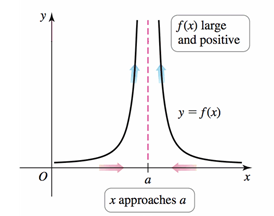
\includegraphics[scale=1]{Fig2_24a}
\end{center}
\end{frame}

% % %
\begin{frame}
\frametitle{Definition of Infinite Limits (cont.)}
Suppose $f$ is defined for all $x$ near $a$.  If $f(x)$ is negative and grows arbitrarily large in magnitude for all $x$ sufficiently close (but not equal) to $a$, we write
\[\lim_{x \to a} f(x) = -\infty\]
and say that \alert{``the limit of $f(x)$ as $x$ approaches $a$ is negative infinity."}
\end{frame}

% % %
\begin{frame}
\begin{center}
\noindent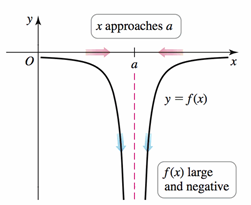
\includegraphics[scale=1]{Fig2_24b} 
\end{center}
\end{frame}

% % %
\begin{frame}
\frametitle{}
\small The definitions work for one-sided limits, too.  

\vspace{0.5pc}
{\bf Example:} Using a graph and a table of values, given $f(x)=\displaystyle\frac{1}{x^2-x}$, determine:
\begin{itemize}
\item[\bf 1.\;] $\displaystyle\lim_{x \to 0^+} f(x)$
\item[\bf 2.\;] $\displaystyle\lim_{x \to 0^-} f(x)$
\item[\bf 3.\;] $\displaystyle\lim_{x \to 1^+} f(x)$
\item[\bf 4.\;] $\displaystyle\lim_{x \to 1^-} f(x)$ 
\end{itemize}
\end{frame}

% % %
\begin{frame}
\frametitle{Definition of Vertical Asymptote}
If any of the following are true:
\begin{itemize}
\item $\displaystyle\lim_{x \to a} f(x) = \pm\infty$,
\item $\displaystyle\lim_{x \to a^+} f(x) = \pm\infty$
\item $\displaystyle\lim_{x \to a^-} f(x) = \pm\infty$
\end{itemize}
then the line $x=a$ is called a {\bf vertical asymptote} of $f$.
\end{frame}

% % %
\begin{frame}
\frametitle{}
{\bf Determining Infinite Limits Analytically:}

\small
\vspace{0.75pc}
Given $f(x)=\dfrac{3x-4}{x+1}$, determine, without using a table or a graph, 

\vspace{0.25pc}
\begin{itemize}
\item $\displaystyle\lim_{x \to -1^+} f(x)$ 
\item $\displaystyle\lim_{x \to -1^-} f(x)$
\end{itemize}
\end{frame}

% % %
\begin{frame}
\frametitle{}
Remember to check for factoring -- what is/are the vertical asymptotes of 
\[f(x)=\frac{3x^2-48}{x+4} ?\]

\vspace{1pc}
What is $\displaystyle\lim_{x \to -4} f(x)$?  
\end{frame}

% % %
\begin{frame}
\frametitle{HW from Section 2.4}
Do problems 7--10, 15, 17--26, 36--37 (pp.\ 81--84 in textbook)
\end{frame}

% % % % %
\begin{frame}
\frametitle{Friday 23 January (Week 2)}
\begin{itemize}
\item For old Calculus materials, see \url{comp.uark.edu/~ashleykw} and look for links under "Courses I've taught".  Last semester's in-class exam solutions are posted in there, too.
\item Quiz solutions are on Dr. Wheeler's course page.
\item Sunday Jan 26:  Computer HWs \#1  and \#2 Due
\end{itemize}
\end{frame}

% % %
\begin{frame}
\subsection[2.5 Limits at Infinity]{$\oint$ 2.5 Limits at Infinity}
\frametitle{$\oint$ 2.5 Limits at Infinity}
Limits at infinity determine what is called the {\bf end behavior} of a function.
\end{frame}

% % %
\begin{frame}
\frametitle{\small Horizontal Asymptotes}
\footnotesize
If $f(x)$ becomes arbitrarily close to a finite number $L$ for all sufficiently large and positive $x$, then we write 
\[\lim_{x \to \infty}f(x)=L.\]
The line $y=L$ is a {\bf horizontal asymptote} of $f$.  

\vspace{3pc}
The limit at negative infinity, $\displaystyle\lim_{x \to -\infty}f(x)=M$, is defined analogously and in this case, the horizontal asymptote is $y=M$.
\end{frame}

% % %
\begin{frame}
\frametitle{\small Infinite Limits at Infinity}
\footnotesize
Is it possible for a limit to be both an infinite limit and a limit at infinity?  (Yes.)

\vspace{2pc}
If $f(x)$ becomes arbitrarily large as $x$ becomes arbitrarily large, then we write 
\[\displaystyle\lim_{x \to \infty}f(x)=\infty.\]  

\vspace{2pc}
(The limits 
$\displaystyle\lim_{x \to \infty}f(x)=-\infty$, $\displaystyle\lim_{x \to -\infty}f(x)=\infty$, and $\displaystyle\lim_{x \to -\infty} f(x)=-\infty$ are defined similarly.)
\end{frame}

% % %
\begin{frame}
\frametitle{\small Infinite Limits at Infinity, cont.}
\small
{\bf Powers and Polynomials:}  Let $n$ be a positive integer and let $p(x)$ be a polynomial.

\vspace{1pc}
\begin{itemize}
\item $n=$ even number: $\displaystyle\lim_{x\to\pm\infty}x^n=\infty$ 

\vspace{1pc}
\item $n=$ odd number: $\displaystyle\lim_{x \to \infty} x^n = \infty$ and $\displaystyle\lim_{x \to -\infty} x^n = -\infty$
\end{itemize}
\end{frame}

% % %
\begin{frame}
\frametitle{}
\footnotesize
\begin{itemize}
\item (again, assuming $n$ is positive)
\[\lim_{x\to\pm\infty}\frac{1}{x^n}=\lim_{x\to\pm\infty}x^{-n}=0\]

\vspace{1pc}
\item For a polynomial, only look at the term with the highest exponent:
\[\lim_{x\to\pm\infty}p(x)=\lim_{x\to\pm\infty}\text{(constant)}\cdot x^n\] 
The constant is called the \alert{leading coefficient}, lc$(p)$.  The highest exponent that appears in the polynomial is called the \alert{degree}, $\deg(p)$.
\end{itemize}
\end{frame}

% % %
\begin{frame}
\frametitle{}
\footnotesize
{\bf Rational Functions:}  Suppose $f(x)=\dfrac{p(x)}{q(x)}$ is a rational function.

\begin{itemize}
\item[{\bf 1.}] If $\deg(p)<\deg(q)$, i.e., \alert{the numerator has the smaller degree}, then 
\[\lim_{x\to\pm\infty}f(x)=0\] 
(also, $y=0$ is a horizontal asymptote of $f$).

\vspace{2pc}
\item[{\bf 2.}] If $\deg(p)=\deg(q)$, i.e., \alert{numerator and denominator have the same degree}, then 
\[\lim_{x\to\pm\infty}f(x)=\dfrac{\text{lc}(p)}{\text{lc}(q)},\] 
and $y=\dfrac{\text{lc}(p)}{\text{lc}(q)}$ is a horizontal asymptote of $f$.
\end{itemize}
\end{frame}

% % %
\begin{frame}
\begin{itemize}
\small
\item[{\bf 3.}] If $\deg(p)>\deg(q)$, \alert{(numerator has the bigger degree)} then 
\[\lim_{x\to\pm\infty}f(x)=\infty\quad\text{or}\quad -\infty\] 
and $f$ has no horizontal asymptote.

\vspace{2pc}
\item[{\bf 4.}] Assuming that $f(x)$ is in \alert{reduced form} ($p$ and $q$ share no common factors), vertical asymptotes occur at the zeroes of $q$.  

\vspace{1pc}
(This is why it is a good idea to check for factoring and cancelling first!)
\end{itemize}
\end{frame}

% % %
\begin{frame}
\frametitle{Exercises}
\small
Determine the end behavior of the following functions (in other words, compute both limits, as $x\to\pm\infty$, for each of the functions):
\begin{itemize}
\item $f(x)=\dfrac{x+1}{2x^2-3}$
\item $g(x)=\dfrac{4x^3-3x}{2x^3+5x^2+x+2}$
\item $h(x)=\dfrac{6x^4-1}{4x^3+3x^2+2x+1}$
\end{itemize}
\end{frame}


% % %
\begin{frame}
\frametitle{}
\small
{\bf Algebraic and Transcendental Functions:}

Determine the end behavior of the following functions.
\begin{itemize}
\item $f(x) = \dfrac{4x^3}{2x^3+\sqrt{9x^6+15x^4}}$ (radical signs appear)

\vspace{1pc}
\item $g(x)=\cos x$ (trig)

\vspace{1pc}
\item $h(x)=e^x$ (exponential)
\end{itemize}
\end{frame}

% % %
\begin{frame}
\frametitle{HW from Section 2.5}
Do problems 9--10, 13--35 odds, 39, 43, 45, 53 (pp.\ 92--93 in textbook)
\end{frame}

\begin{comment}
\end{comment}

\end{document}